\section{Modern cosmology}
\label{sec:cosmo_model}

Modern cosmology, or simply cosmology, is the study of the largest-scale structures and dynamics of the Universe as a whole and is concerned with fundamental questions about its formation, evolution, and ultimate fate. Cosmology as a science originated with the Copernican principle, which states that celestial bodies obey identical physical laws to those on Earth. During the 20th century, Cosmology developed widely with Albert Einstein's General Theory of Relativity, and with better astronomical observations of extremely distant objects. Currently, the most accepted cosmological model is called $\Lambda$ Cold Dark Matter ($\Lambda$CDM).

\subsection{The geometry of the Universe}
The cosmological principle asserts that the distribution of matter-energy in the universe at large scales ($\gtrsim$100Mpc) is homogeneous and isotropic, so there is no preferred direction on the sky. According to the General Theory of Relativity, the unique metric compatible with this principle is the Friedmann-Lemaitre-Robertson-Walker (FLRW) metric, whose space-time line element is:  
\begin{equation}
ds^2 = -c^2dt^2 + a(t)^2dx^2,
\label{eq:space-time_line}
\end{equation}
where $-cdt$ is the temporal contribution with $c$ the speed of light and $a(t)dx$ the spatial, which is the product of a time-dependent scale factor $a(t)$ and a comoving space line element $dx$. Since only the product $a(t)dx$ has a physical meaning of distance, the absolute value of $a$ is arbitrary and it is usually taken equal to 1 today. If the scale factor grows in time ($\dot{a}>0$), spatial distances will grow as well, so in that case, we will say that the Universe is expanding. The FLRW metric admits three different kinds of spatial curvature for the whole Universe: hyperbolic, flat and spherical. In the case that it is flat, which seems to be in good agreement with the current Cosmic Microwaves Background (CMB) radiation observations~\citep{komatsu2009, Ade2013}, it can be written in spherical coordinates $\lbrace r, \theta, \varphi \rbrace$ as:
\begin{equation}
dx^2 \equiv dr^2 + r^2d\Omega^2,
\end{equation}
where $d\Omega^2 \equiv d\theta^2 + \sin^2\theta d\varphi^2$ is the differential solid angle. From now on, we will consider that the Universe is spatially flat and all equations we will show will be valid under this assumption.

\subsection{Cosmological Redshift}
When light (or any electromagnetic radiation) coming from a distant celestial object, such as a galaxy, travels across the space of an expanding Universe, all its wavelengths suffer an elongation due to the growth of distances. This effect is called cosmological redshift and it is equivalent to the elongation of the wavelengths that any wave suffers when it comes from a source which is moving away (Doppler effect). It can be quantified as: 
\begin{equation}
z \equiv {\lambda_{obs} - \lambda_{em} \over \lambda_{em}},
\label{redshift}
\end{equation} 
where $\lambda_{obs}$ is the wavelength of the light when is received by the observer and $\lambda_{em}$ when it was emitted by the source. From now on, we will simply refer to redshift when we actually refer to cosmological redshift. It is easy to show through the geodesic equation (movement equation) in a FLRW metric that there is a relation between the scale factor $a$ at the time when light was emitted and how redshifted the light is today. 
\begin{equation}
1 + z = {1 \over a(t)}
\label{z2a}
\end{equation} 
In Fig.~\ref{fig:sdss_filt} we show the spectrum of the star Vega ($\alpha$-Lyr) as reference at three different redshifts: 0, 0.4, 0.8 (note that such redshifts for a star in the Milkyway are not real, but only illustrative). As it is redshifted, its spectral features, such as the prominent absorption valleys, shift towards higher (redder) wavelength and they are stretched.
\begin{figure}
\centering
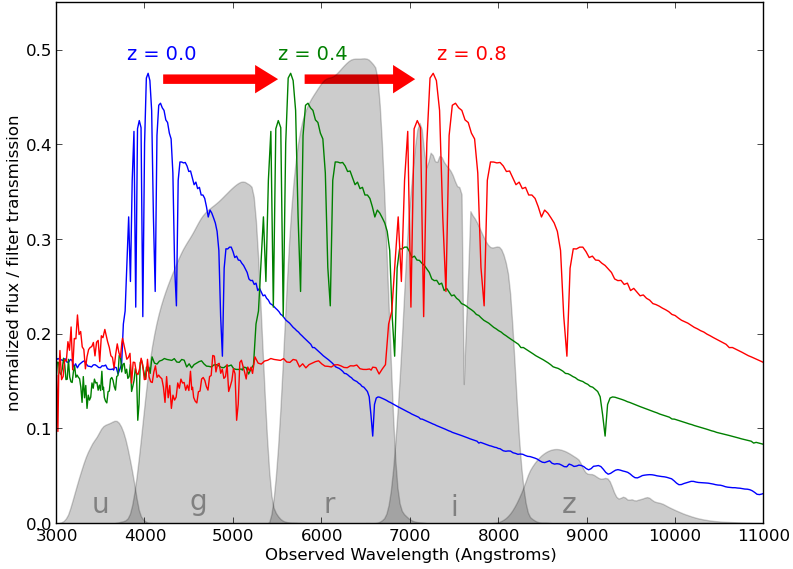
\includegraphics[width=110mm]{./plots/plot_sdss_filters.png}
\caption{On the foreground, the spectrum of the star Vega ($\alpha$-Lyr) as a reference at three different redshifts: 0 (blue), 0.4 (green) and 0.8 (red). As it is redshifted, its spectral features, such as the prominent absorption valleys, move towards higher wavelength and they are stretched. The spectra have been normalized to have the same height. On the background, the throughput $R(\lambda)$ of the SDSS broad-band photometric system $ugriz$ \citep{Fukugita1996}. (Plot generated with the public script at \url{http://www.astroml.org/sklearn_tutorial/_downloads/plot_sdss_filters.py}.)}
\label{fig:sdss_filt}
\end{figure}

\subsection{The evolution of the universe}
Assuming that the matter-energy content of the universe at large scales can be described as a perfect fluid, which follows the state equation $P = \omega \rho$, where $P$ is the pressure, $\rho$ the density and $\omega$ is the state parameter of the fluid that relates them, the gravitational field equation gives us the temporal evolution $a(t)$ of the FLRW metric in its differential form called the Friedman equation:
\begin{equation}
H \equiv {\dot{a} \over a} = H_0\sqrt{\sum_\omega \Omega_{\omega}a^{-3(1+w)}},
\label{eq:friedman}
\end{equation} 
where $H_0 \sim 70 (km/s)/Mpc$ is the Hubble constant, which is the value of the so called Hubble parameter $H$ today. The sum inside the root is over all the different perfect fluids that fill the universe, such as non-relativistic matter (dust, gas, cold dark matter\footnote{Cold dark matter (or CDM) is a hypothetical form of matter that interacts very weakly with electromagnetic radiation (dark) and most of whose particles move slowly compared to the speed of light (cold). Its presence can be only detected through its gravitational or weak interactions with ordinary matter and radiation.}) ($\omega \sim 0$), radiation ($\omega=1/3$), etc., and $\Omega_\omega \equiv \rho / \rho_c$ are their densities relative to the critical density $\rho_c \equiv 3H^2_0 / 8\pi G$ today, where $G\sim6.67\cdot10^{-11}N\cdot(m/kg)^2$ is the gravitational constant. Relative densities must fulfill $\sum_\omega \Omega_\omega =1$ in a flat Universe. We refer to the collection of parameters $\lbrace \Omega_\omega, H_0 \rbrace$ as the cosmology of the Universe, which determines the evolution and destiny of its space-time metric. Using the spatial part of the FLRW space-time line element at (\ref{eq:space-time_line}) and the definition of $H$, it can be deduced that the receding velocity $v$ of a galaxy in an expanding universe ($\dot{a}>0$) is $v = Hd$, where $d$ is the physical distance to the galaxy. Edwin Hubble proved, by measuring the distance and the receding velocity of 22 galaxies (see Fig.~\ref{fig:hubble_diagram}), that this is the case for our Universe \citep{Hubble1929}. Many times cosmological parameters are given in terms of the normalized Hubble parameter $h\equiv H_0/100(km/s)/Mpc\sim0.7$. Also note that when $c>Hd$, where $c$ is the speed of light, the receding galaxy becomes causally disconnected to the observer, which defines a causal horizon.
\begin{figure}
\centering
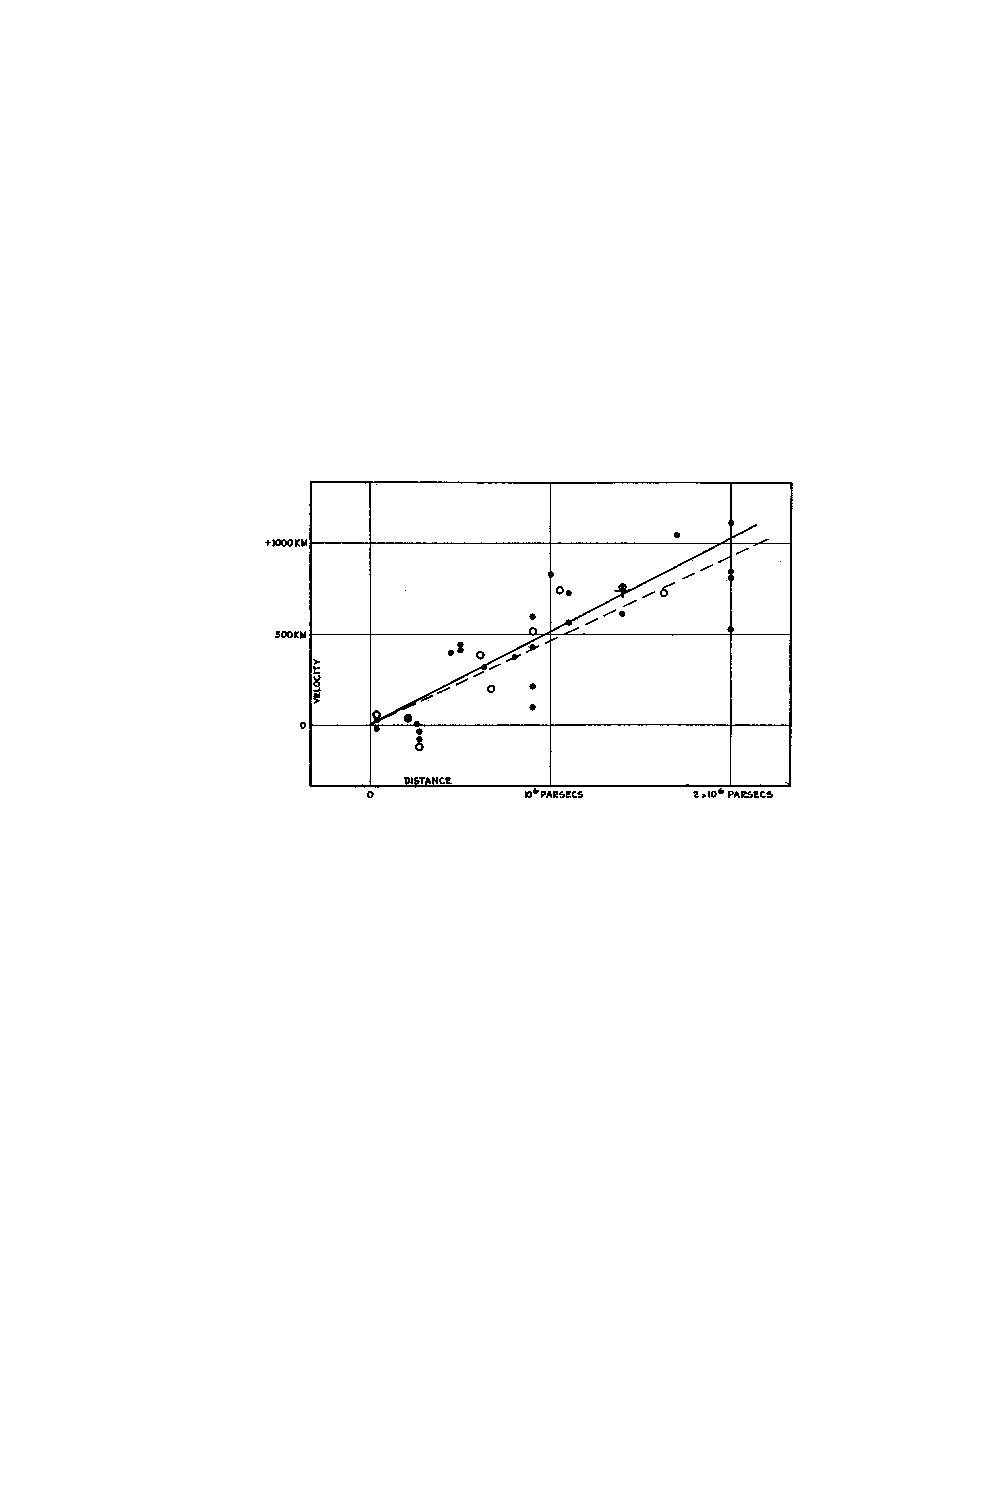
\includegraphics[width=110mm]{./plots/Hubblediagram.pdf}
\caption{Original scatter plot from \citet{Hubble1929} of the velocity $v$ (km/s) vs. distance $d$ (pc) of 22 galaxies that proves that the universe is expanding. According to this, galaxies follow a lineal relation $v=Hd$.} 
\label{fig:hubble_diagram}
\end{figure}

Besides the expansion rate of the universe given by $H$, another interesting quantity is the deceleration parameter $q$ defined as:
\begin{equation}
q \equiv -{\ddot{a} \over aH} = {1 \over 2} \sum_\omega \Omega_{\omega}{(1+3w)}.
\label{eq:deceleration}
\end{equation} 
According to this definition, a universe basically made of ordinary matter ($\omega \sim 0$) would have a deceleration parameter $>0$, that is, the expansion rate would be decelerating due to the gravitational attraction. However, any unknown component with $\omega < -1/3$ would do the opposite, accelerate the expansion rate. In the next subsection, we will see that this is actually the case.

\subsection{Cosmological distances}
\label{sec:distances}
The radial comoving distance $r$ that light traveled since it left the source until it arrives to us can be computed by equating the space-time line element in (\ref{eq:space-time_line}) to 0. Note that in spherical coordinates light only travels radially respect to us ($d\Omega = 0$ and $dx = dr$). Using the definition of the Hubble parameter in (\ref{eq:friedman}) and the relation between the redshift and the scale factor in (\ref{z2a}), $r$ can be expressed as 
\begin{equation}
r(z) = c \int_0^{z} {dz' \over H(z')},
\label{comoving_distance}
\end{equation}
where the integral goes from redshift 0, when light is observed, to redshift $z$, when it was emitted. If we want to know the equivalent current physical distance, we only have to multiply by the scale factor today.

In astronomy, distances to celestial objects have been usually determined by measuring either its apparent brightness (flux $F$) on the sky when its absolute luminosity $L$ is well-known (standard candles), or the apparent size (angle subtended $\theta$) on the sky when its actual size $\ell$ is also well-know (standard rulers). It is easy to see through geometrical and energy conservation arguments that the luminosity distance defined as follows is related to the redshift $z$ as
\begin{equation}
D_L \equiv \sqrt{L \over 4 \pi F}  = r(z) (1+z),
\label{eq:DL}
\end{equation}
while the angular distance is
\begin{equation}
D_A \equiv {\ell \over \theta} = {r(z) \over (1+z)}.
\label{eq:DA}
\end{equation}
These two relations are very important because they allow us to constrain the cosmology of our Universe by simply measuring the relation of two physical quantities such as the flux $F$ or subtended angle $\theta$ of standard candles or rulers respectively with its redshift $z$. Moreover, if we have enough redshift precision, we will be able to measure the radial size (the difference in redshift $\delta z$ between the nearest and the farthest part) of a standard ruler that is aligned with the line of sight. With this, we see by differentiating (\ref{comoving_distance}) that we can directly measure the Hubble parameter as $H(z) = c \delta z / \ell$. If the standard ruler is perfectly spherical with diameter $\ell$, we can measure $D_V(z)$~\citep{Eisenstein2005}, a hybrid distance that takes into account both contributions:
\begin{equation}
D_V \equiv \left((1+z)^2 D_A^2 {cz \over H(z)} \right)^{1/3}.
\label{eq:DV}
\end{equation}

Typical standard candles in observational cosmology are type Ia Supernovae (SNIa), which are very energetic nuclear explosions that occur when a white dwarf star in a binary system accreats material from the companion until surpasses the Chandrasekhar's limit. When they are produced in another galaxy, they can shine brighter than the host galaxy itself, so they can be seen at very large distances (or very high redshifts). Moreover, after some corrections, they all appear to have very similar absolute luminosities. In the late 1990’s two independent teams, the Supernova Cosmology Project~\citep{Perlmutter1999} and the High-$z$ SN Search~\citep{Riess1998} measured the relation between the luminosity distance $D_L$ of high-$z$ SNIa ($z>0.15$) and their redshift (see Fig.~\ref{fig:hubble_diagram_sn1a}). They found out that (\ref{eq:DL}) fits best the data when the cosmology is $\lbrace \Omega_{CDM} \sim 0.3, \Omega_\Lambda \sim 0.7 \rbrace$, where $\Lambda$ is an unknown component of the universe, such as a cosmological constant or dark energy, with state parameter $\omega_\Lambda \sim -1$. According to this result the deceleration parameter $q$ defined in (\ref{eq:deceleration}) is negative, so the universe expansion rate is not decelerating, as was originally thought, but accelerating.
\begin{figure}
\centering
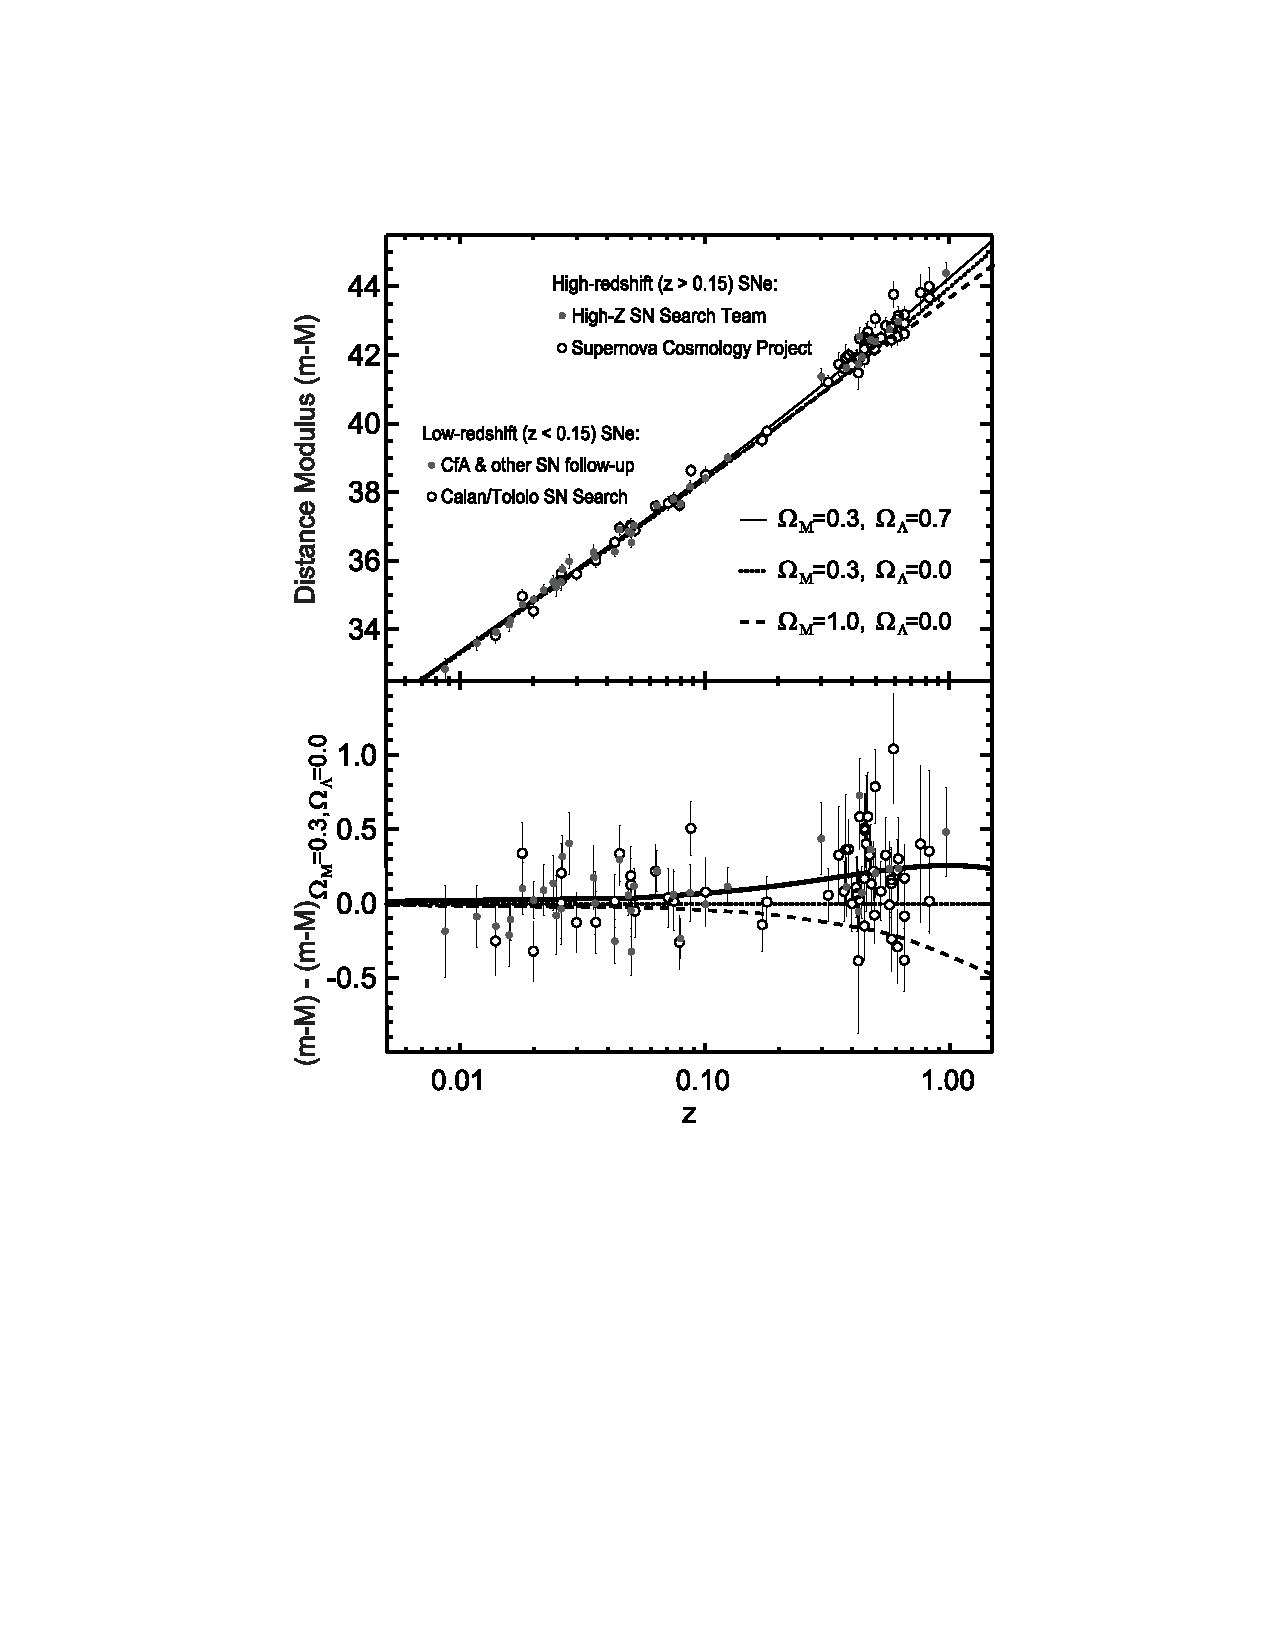
\includegraphics[width=90mm]{./plots/perlmutter_riess_hubble_diagram.pdf}
\caption{Top: The scatter plot of the distance modulus, defined in subsection~\ref{sec:absolute_mag} as $m-M \equiv 5\log_{10}(D_L / 10pc)$, vs. the redshift of low-$z$ SNIa ($z<0.15$) from the Calan/Tololo SN Search \citep{Hamuy1993} and other SN surveys, and high-$z$ SNIa ($z>0.15$) from the High-$z$ SN Search~\citep{Riess1998} and the Supernova Cosmology Project~\citep{Perlmutter1999}. Bottom: The residuals of the distances relative to a $\Omega_{CDM}=0.3$, $\Omega_\Lambda=0.0$ Universe. The best fit to data occurs with $\Omega_{CDM}=0.3$ and $\Omega_\Lambda=0.7$, which implies that the Universe expansion rate is accelerating. Figure from \citet{Perlmutter2003}.}
\label{fig:hubble_diagram_sn1a}
\end{figure}

A typical standard ruler in observational cosmology is the Baryon Acoustic Oscillation (BAO). Back ($z>1100$) when Universe was denser and hotter ($T\gg13.6$~eV) enough that hydrogen atoms could not form, the plasma of baryons and photons continuously interacting through Thomson scattering ($p+e^- \rightleftharpoons H+\gamma$) created a pressure on that medium thorugh which acoustic waves traveled at the speed $c_s = \sqrt{\partial p /\partial \rho}=c/\sqrt{3(1+R)}$, where $R \equiv 3\rho_b / 4\rho_\gamma$ and, $\rho_b$ and $\rho_\gamma$ are the densities of baryons and photons respectively at that time. The Universe was expanded and cooled down until the recombination era when hydrogen atoms could start to form ($p+e^- \Rightarrow H+\gamma$), so the pressure on the medium vanished and traveling waves stalled at a comoving distance
\begin{equation}
r_d \sim c_s \int_{1100}^{\infty} {dz \over H(z)} \sim 150\ \rm Mpc
\end{equation}
from the initial overdensity where they were created, where $\infty$ denotes the beginning of the Universe. Additionally, photons started to move freely across space creating what we now observe as the Cosmic Microwaves Background (CMB) radiation. Recent accurate measurements of the CMB with the Plank mission show that, in fact, $r_d=147.49 \pm 0.59$Mpc at $z_d = 1059.25\pm0.58$ \citep{Ade2013}. Later, these secondary overdensities, as well as the initial ones, seeded the formation of galaxies resulting in an excess of galaxies separated by $\sim150$~Mpc from each other. \citet{Eisenstein2005} was the first to detect this preferred distance by measuring the 3D redshift-space correlation function $\xi(s)$ (black points in Fig.~\ref{fig:xi_bao}) with the SDSS survey (see subsection~\ref{sec:sdss}) LRG\footnote{Luminous Red Galaxies (LRGs) are luminous intrinsically red galaxies consistent with large/giant elliptical galaxies.} spectroscopic galaxy sample. Note, from Fig.~\ref{fig:xi_bao}, that besides the exponential decreasing shape of $\xi(s)$ there is a small bump at $\sim150$~Mpc corresponding to the BAO signature.
\begin{figure}
\centering
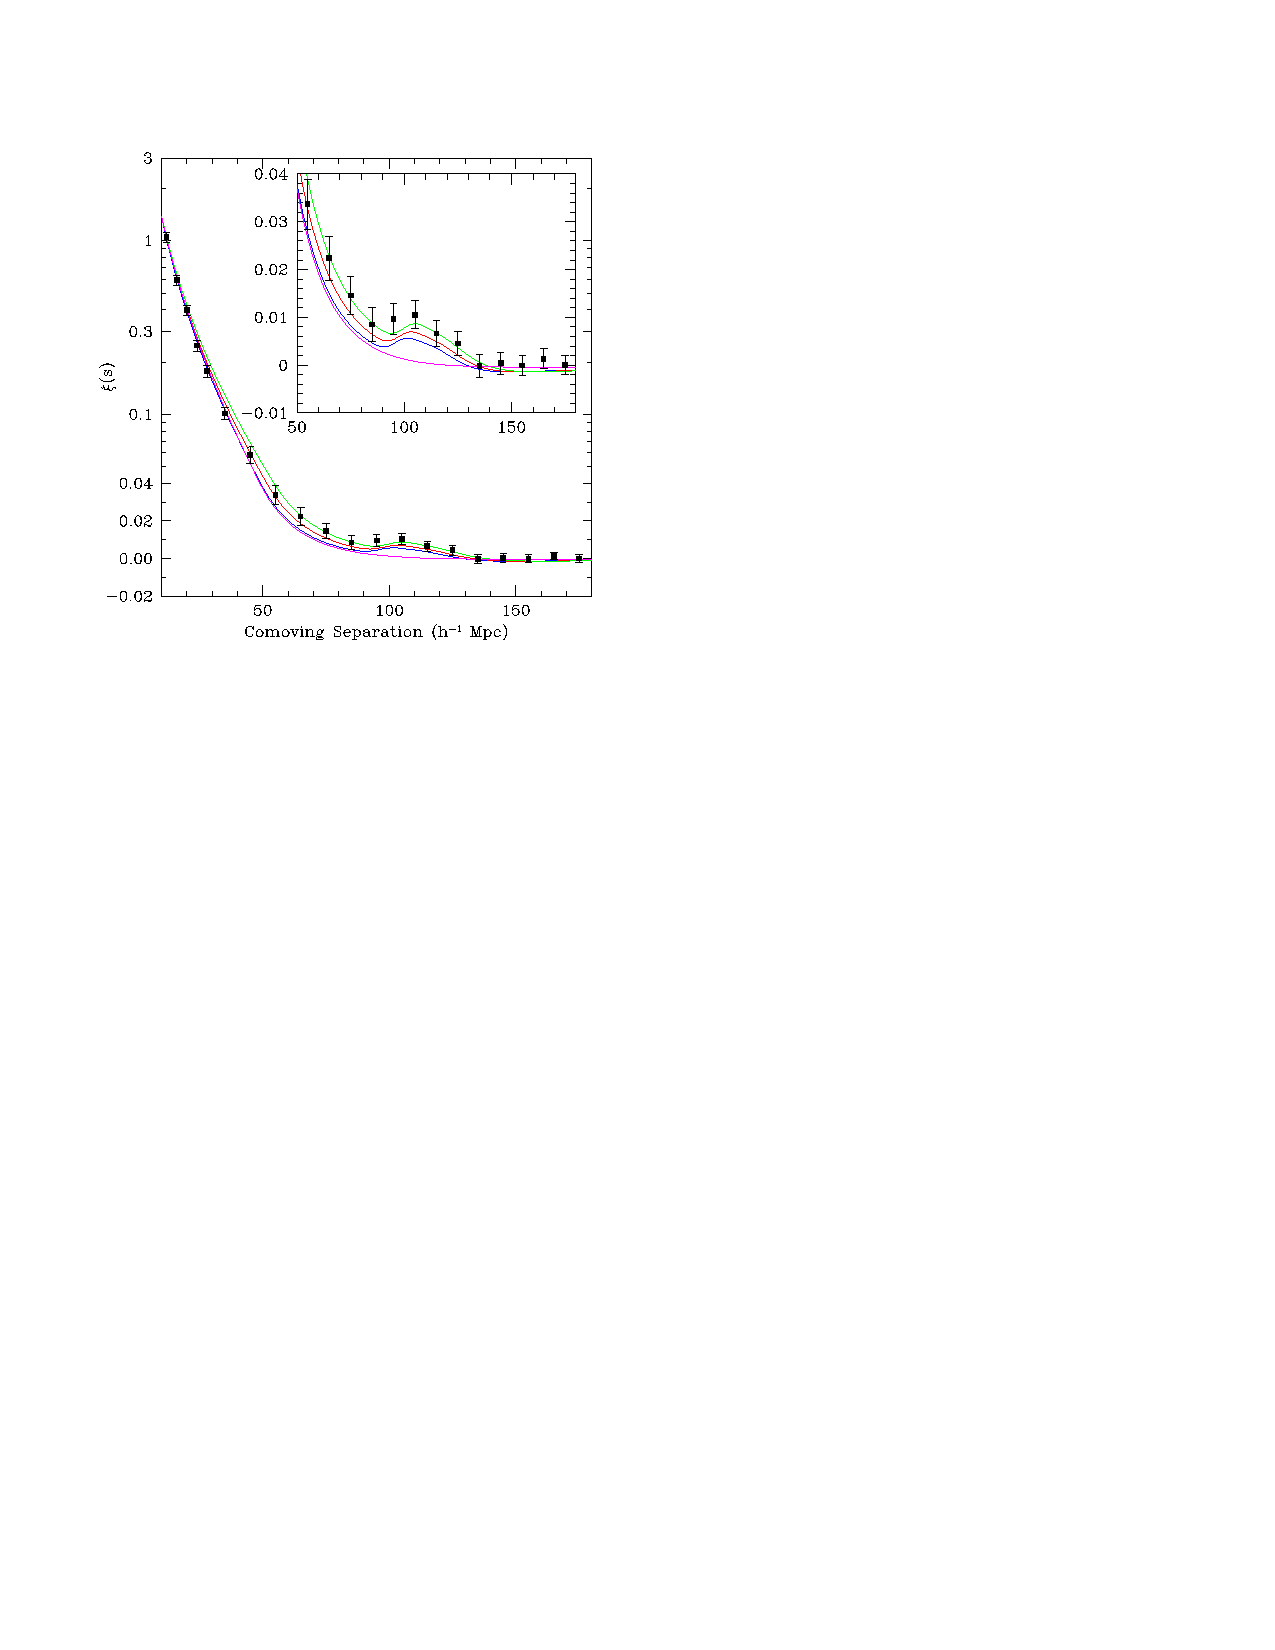
\includegraphics[height=90mm]{./plots/bao_eisenstein.pdf} 
\caption{The large-scale redshift-space correlation function $\xi(s)$ of the SDSS LRG spectroscopic sample \citep{Eisenstein2005}. Note that the vertical axis mixes logarithmic and linear scales. The inset shows an expanded view with a linear vertical axis. Points correspond to measured data, while lines correspond to different models. The BAO peak is clearly seen at 100~Mpc/h $\sim$ 150~Mpc. The magenta line is a model which does not include the BAO signature.}
\label{fig:xi_bao}
\end{figure}
During the last fifteen years, detections of BAO with other samples have been carried out. In Fig.~\ref{fig:DV_bao} we show a Hubble diagram $D_V$ vs. $z$ for different measurements at different redshifts with the spectroscopic samples: 2dFGRS (\citet{Colless2001}, $z=0.2$), SDSS (\citet{York2000}, $z=0.2$ and $z=0.35$) and WiggleZ (\citet{Drinkwater2010}, $z=0.6$). Two predicted curves for two different cosmologies, $\Lambda CDM\equiv\lbrace \Omega_{CDM} \sim 0.3, \Omega_\Lambda \sim 0.7 \rbrace$ (solid line) and a pure CDM Universe $\lbrace \Omega_{CDM}\sim 0.3, \Omega_\Lambda \sim 0 \rbrace$ (dashed), are also shown. Data are in agreement with the $\Lambda CDM$ model, consistent with the SNIa results.
\begin{figure}
\centering
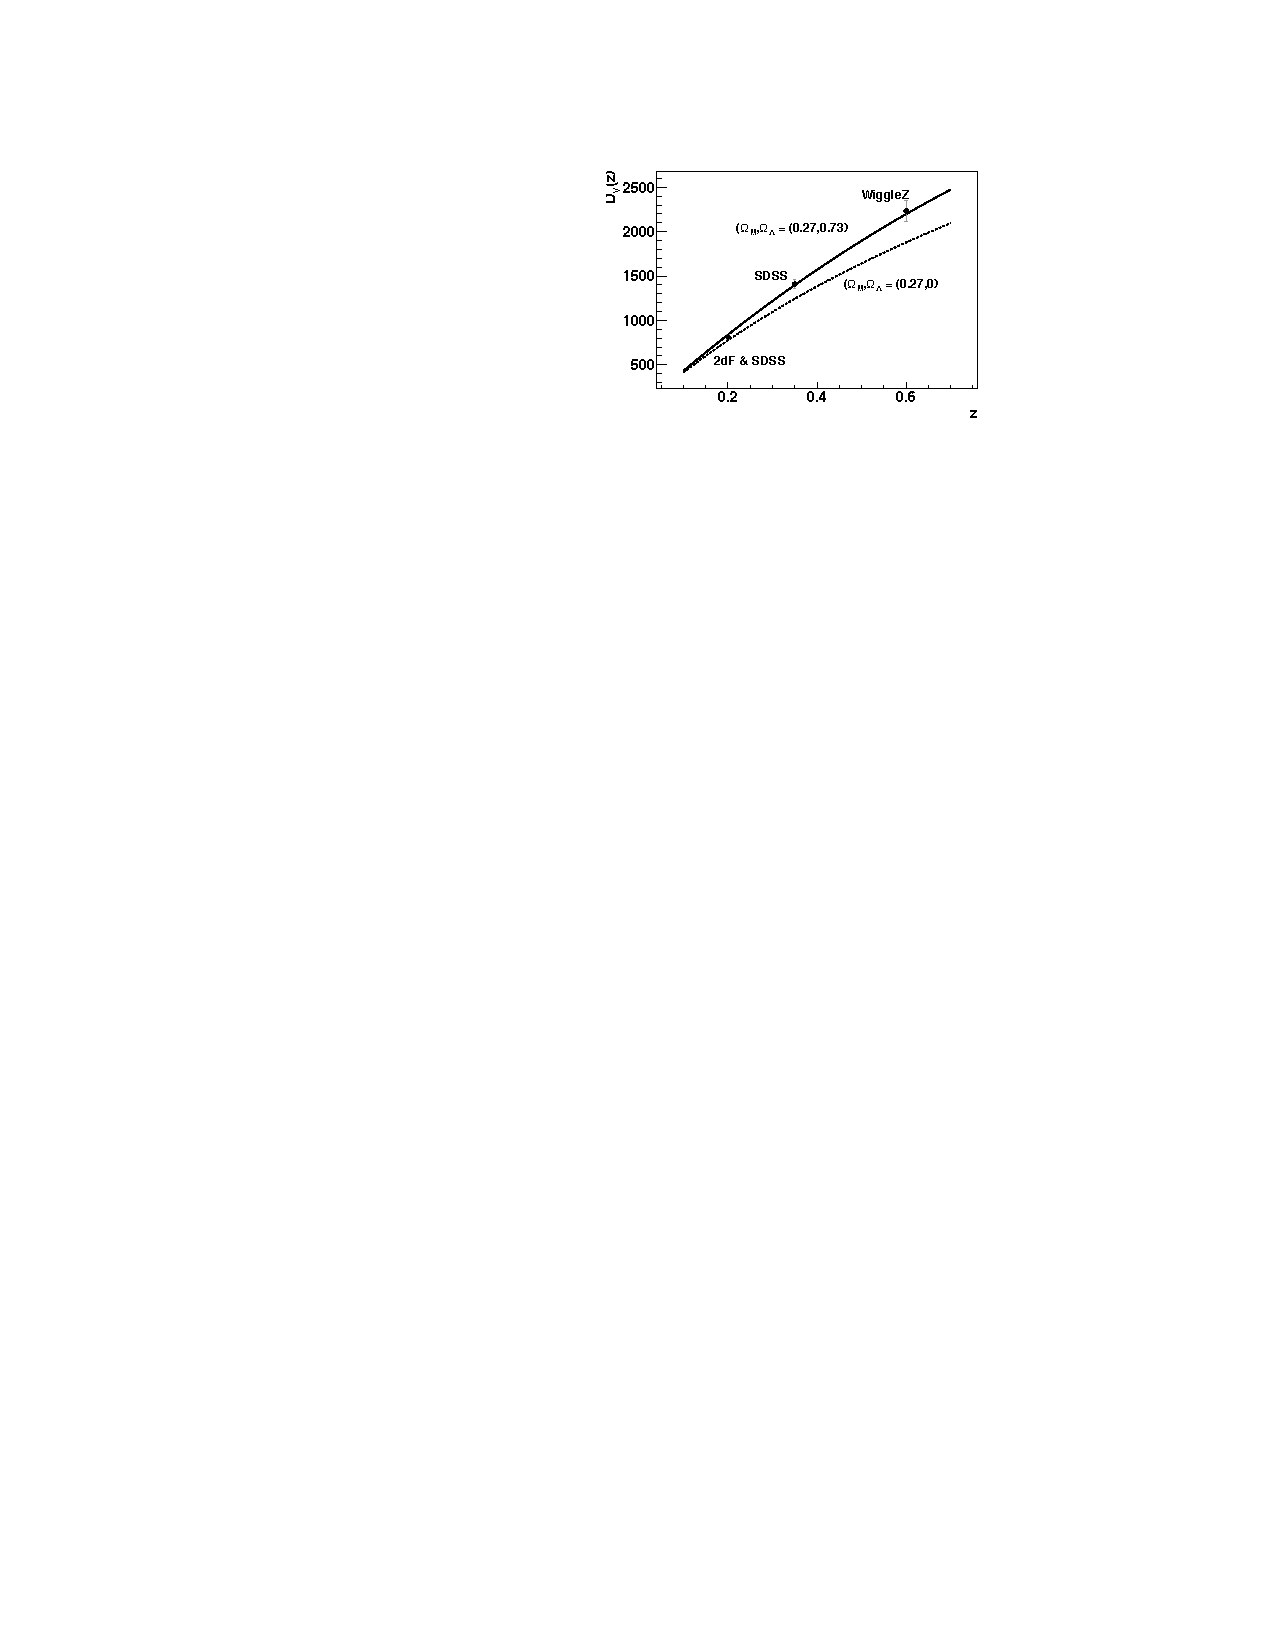
\includegraphics[height=75mm]{./plots/dv_bao.pdf}
\caption{The Hubble diagram $D_V(z)$, defined in (\ref{eq:DV}), vs. redshift obtained by measuring the BAO signature in a combination of the transversal and radial directions with the spectroscopic samples: 2dF (\citet{Colless2001}, $z=0.2$), SDSS (\citet{York2000}, $z=0.2$ and $z=0.35$) and WiggleZ (\citet{Drinkwater2010}, $z=0.6$). The data points agree with the prediction corresponding to a cosmology $\Lambda CDM \equiv\lbrace \Omega_{CDM} \sim 0.3, \Omega_\Lambda \sim 0.7 \rbrace$ (solid line). Figure from \citet{Astier2012}.}
\label{fig:DV_bao}
\end{figure}

Nowadays, most of the observational cosmology is focused into determine precisely the cosmology of our Universe. Current cosmological proves agree that the Universe is very close to flat and basically made of cold dark matter ($\omega_{CDM} = 0$) with relative density $\Omega_{CDM} \sim 0.3$ and some unknown ingredient called Dark Energy ($\omega_\Lambda \sim -1$) with $\Omega_\Lambda \sim 0.7$, responsible of the expansion rate acceleration. The Friedman equation for a Universe like this is reduced to:
\begin{equation}
H(z) = H_0 \sqrt{\Omega_{CDM}(1+z)^3 + \Omega_\Lambda}
\end{equation}
where $a$ on the right of equality (\ref{eq:friedman}) has been replaced by (\ref{z2a}). It is usually referred as the $\Lambda$CDM Universe. In this paradigm, ordinary matter (baryonic matter) would also account for $\lesssim5\%$ of the total content.

\subsection{Large-Scale Structure (LSS)}
\label{sec:lss}

At scales $<$100Mpc Universe can not be considered homogeneous since it presents structures such as galaxy clusters, voids and filaments, as shown in Fig.~\ref{fig:2dfzcone}. At those scales the FLRW metric is no longer valid however, the Newtonian description of gravity is a good approximation. Consider that small deviations at different positions and times on the density $\rho(\vec{x},t)$ of the perfect fluid can be quantified as:
\begin{equation}
\delta(\vec{x}, t) \equiv {\rho(\vec{x},t) \over \bar{\rho}(t)} - 1,
\end{equation}
which is called the density contrast, with $\bar{\rho}$ the average density. According to the Newtonian potential and mass conservation, the evolution in time of these fluctuations in an expanding universe is given by the second order harmonic differential equation:
\begin{equation}
\ddot{\delta} + 2H\dot{\delta} - {3 \over 2}H^2 \delta = 0,
\label{eq:diff_delta}
\end{equation}
where $H$ is the Hubble parameter defined in (\ref{eq:friedman}). The solution, $\delta(\vec{x},t) = D^{\pm}(t)\delta(\vec{x})$, consists of a growing ($+$) and a decaying ($-$) mode, with a completely decoupled temporal and spatial parts. Since eventually the growing mode dominates, we simply write the solution as 
\begin{equation}
\delta(\vec{x},z) = D(z)\delta(\vec{x}),
\label{eq:growth_factor}
\end{equation}
where $D(z)$ ($t$ has been replaced by $z$ through (\ref{z2a})) is called the linear growth factor and gives the evolution in redshift (time) of the initial spatial perturbation $\delta(\vec{x})$.
Clearly, the evolution of these perturbations and, therefore, the evolution of the large-scale structure is not only driven by the gravitational pull of the perturbations themselves, but also by the evolution of the space-time metrics of the whole Universe. This allows cosmologists trace to the story of $a(t)$ and determine the cosmology of the Universe by observing how structures have formed and evolved.
\begin{figure}
\centering
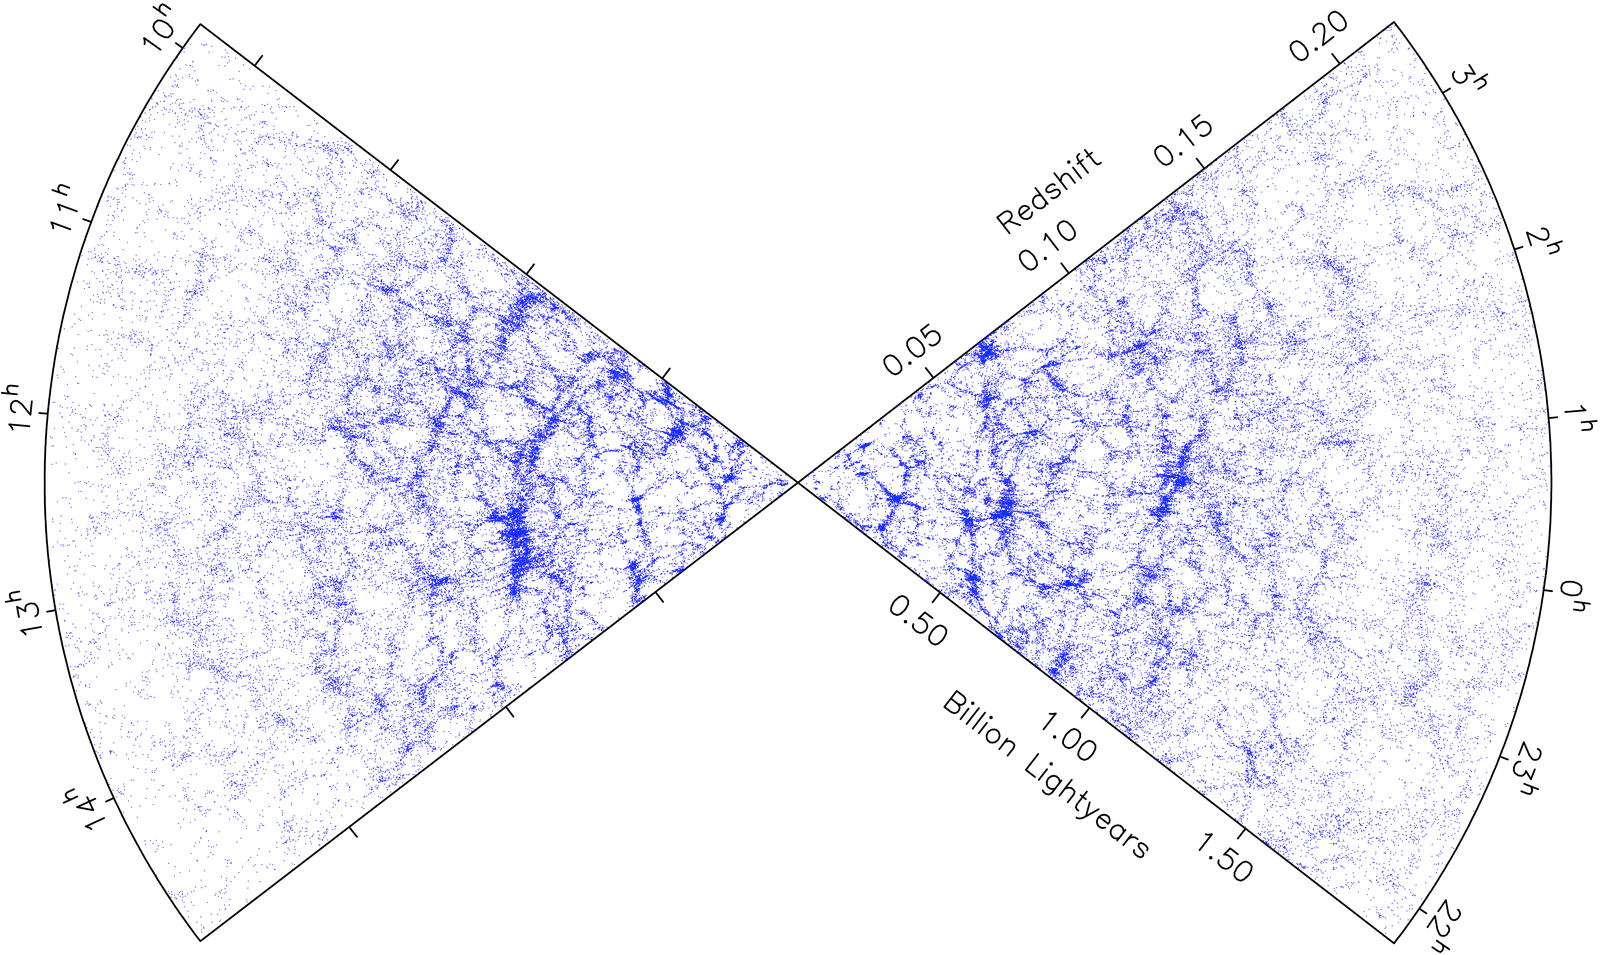
\includegraphics[width=130mm]{./plots/2dFzcone_big.png}
\caption{The distribution of $\sim 0.2$~million galaxies (blue) observed with the 2dFGRS survey \citep{Colless2001} in two slices $4$~deg thick, centered at declination $-2.5$~deg in the North Galactic Pole and $-27.5$~deg in the South Galactic Pole. Although the distribution of matter at large scales ($>100$~Mpc) can be considered as homogeneous and isotropic, at lower scales galaxies form structures such as galaxy clusters, voids and filaments.}
\label{fig:2dfzcone}
\end{figure}
Since the formation of galaxies is seeded by cold dark matter overdensities (the most dominant component of matter), the easiest way to trace the distribution of cold dark matter is by looking at the three-dimensional position of galaxies on the sky. However, in \citet{Fry1993} it was shown that there is a bias $b$ between the fluctuations of the galaxy density contrast $\delta_G$ and the CDM density contrast $\delta$ defined as follows
\begin{equation}
\delta(\vec{x},z)_G = b(z) \delta(\vec{x},z),
\label{eq:bias}
\end{equation}
where $b$ can depend on the redshift.

Cosmologists are not actually interested in the value of $\delta(\vec{x},z)$, but in their statistical properties. For this purpose, they compute the two-point correlation function in a given volume $V$
\begin{equation}
\xi(\vec{r}) = \langle \delta(\vec{y}) \delta(\vec{y}+\vec{r}) \rangle_V = {1 \over V}\int \delta(\vec{y})\delta(\vec{y}+\vec{r})dV_y,
\end{equation}
which, assuming isotropy, gives the differential probability $dP = \bar{\rho}^2(1+\xi(r))dV_ydV_{y+r}$ to find a fluctuation of size $\delta (\vec{y})$ a distance $r=|\vec{r}|$ away from another fluctuation of size $\delta (\vec{y}+\vec{r})$. Even more interesting is the Fourier transform of the 2-point correlation function $\xi(\vec{r})$:
\begin{equation}
P(\vec{k}) = \int \xi(\vec{r})e^{i\vec{k}\vec{r}}d^3k,
\end{equation}
which is called the matter power spectrum. Note that the density contrast, $\delta({\vec{x}})$, can also be Fourier transformed to $\delta({\vec{k}})$, so that the matter power spectrum can be computed simply as $P(\vec{k})=V|\delta(\vec{k})|^2$. Most inflationary\footnote{Inflation is a cosmological model for the early universe that predicts an extremely rapid exponential expansion driven by a negative-pressure vacuum energy density. Initial quantum fluctuations become macroscopic on this process seeding the current inhomogeneities observed on the matter distribution.} theories predict a primordial density contrast whose amplitude $\delta(\vec{r})$ is isotropic and homogeneously Gaussian distributed (observationaly confirmed in \citet{komatsu2009}), as well as a power spectrum $P(k) \propto k$ (Harrison-Zeldovich power spectrum) that is scale-invariant. However, the shape of $P(k)$ at low scales is strongly modified by the radiation dominated era ($\Omega_{rad} \gg \Omega_{matter}$) where perturbations whose wavelength scale $\lambda$ was smaller than the causal horizon had a linear growth factor $D(z)$ that remains constant until the matter dominated era due to the suppression caused by the pressure of radiation (see \cite{Dodelson2003} for a more detailed explanation). This results in the power spectrum, shown in Fig.~\ref{fig:pk}, which asymptotes to $P(k)\sim k$ for small $k$, and behaves as $P(k)\sim k^{-3}$ for large $k$, with a peak at $k^\ast \sim 2 \times 10^{-2} h\ \rm Mpc^{-1}$ corresponding to $\lambda^\ast\sim 350 h^{-1}\ \rm Mpc$.
\begin{figure}
\centering
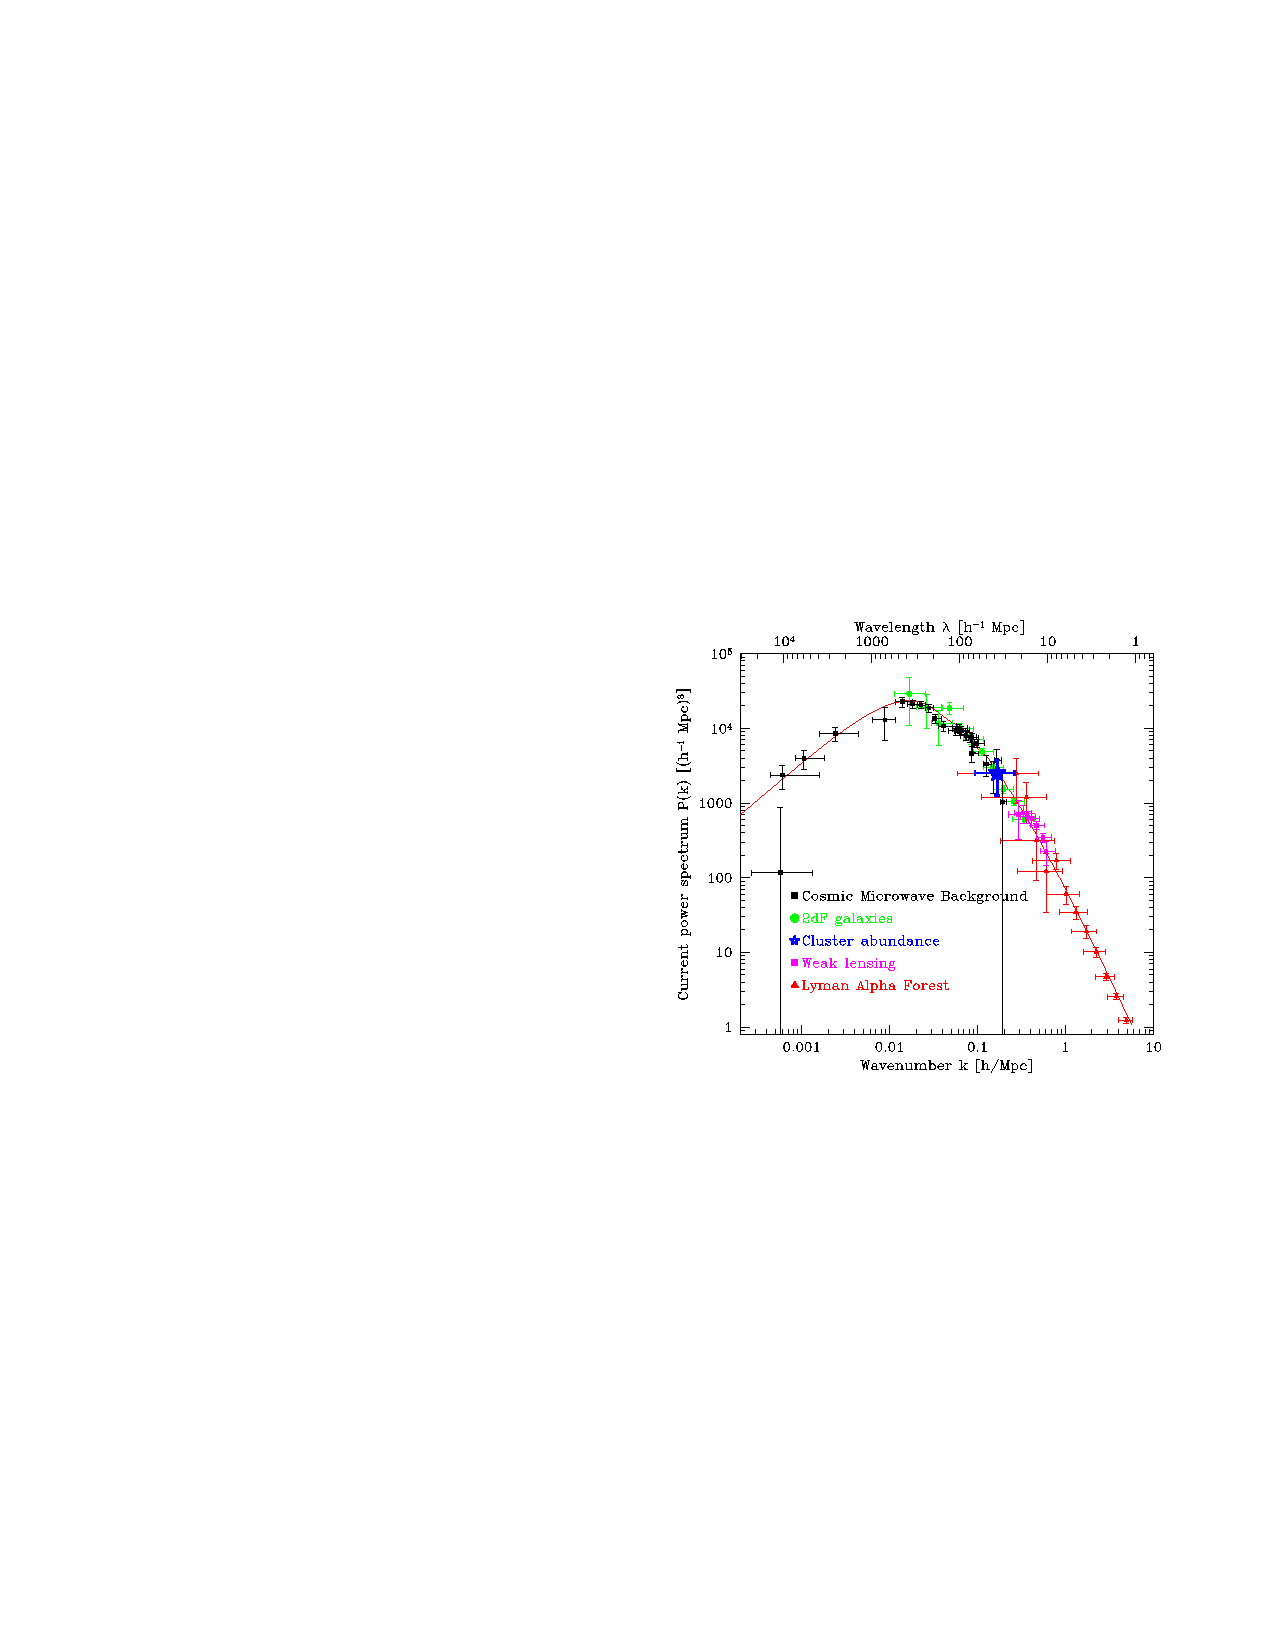
\includegraphics[width=110mm]{./plots/pk.pdf}
\caption{Matter power spectrum $P(k)$ versus wavenumber extrapolated to $z=0$, from various measurements of cosmological structure. The best fit $\Lambda CDM$ model is shown as a solid line. Figure from \citet{Tegmark2002b}.}
\label{fig:pk}
\end{figure}

We typically measure distances to galaxies through the relation between their redshift and distance given by the Hubble law. However, peculiar radial velocities of galaxies not associated with the expansion flow can cause distortions on the measurement of the cosmological redshift. The most obvious example of this is the Fingers-of-God effect \citep{Bahcall1986}, where long thin filaments in the distribution of galaxies in redshift space point directly back at the observer due to the addition of the random peculiar velocities of galaxies, given by the virial theorem\footnote{The virial theorem relates the average over time of the total kinetic energy of a stable system consisting of $N$ particles, bound by potential forces, with that of the total potential energy.}, in the radial direction within a galaxy cluster. Another important redshift-space distortion is the Kaiser effect \citep{Kaiser1984}, which is more subtle and difficult to quantify. The Kaiser effect describes the peculiar velocities of galaxies bound to a central mass as they undergo infall. This differs from the Fingers-of-God in that the peculiar velocities are coherent, not random, towards the central mass. According to this effect, in the large-scale linear regime ($\delta \ll 1$) and the plane-parallel approximation (where galaxies are taken to be sufficiently far away from the observer that the displacements induced by peculiar velocities are effectively parallel), the distortion caused by coherent infall velocities takes a particularly simple form in Fourier space:
\begin{equation}
\delta^s(\vec{k})=(b+f\mu^2_{\vec{k}})\delta(\vec{k}),
\label{eq:kaiser}
\end{equation}
where $\mu$ is the cosine of the angle between $\vec{k}$ and the line-of-sight, $b$ is the bias described in (\ref{eq:bias}), the subscript $s$ indicates redshift space, and $f$ is the velocity growth factor defined as
\begin{equation}
f(z)\equiv{d\ln D \over d \ln a}={\dot{\delta} \over \delta}\equiv\Omega_{CDM}^\gamma(z),
\end{equation}
and $\gamma$, the gravitational growth index \citep{Linder2008}.

In many cases what is measured is the angular galaxy-galaxy cross-correlation function of the galaxies at different redshifts. It can be predict by considering the projected spatial galaxy contrast in a redshift bin $i$
\begin{equation}
\delta_{G_i}(\hat{n}) = \int dz N_i(z) \delta (\hat{n}, z),
\end{equation}
where $N_i(z)$ is the redshift distribution in the redshift bin $i$ and $\hat{n}$ is some unitary vector pointing to some direction on the sky. Then, the angular cross-correlation between two redshift bins $i$ and $j$ is
\begin{equation}
\omega_{G_iG_j} (\theta) \equiv \langle \delta_i (\hat{n}) \delta_j(\hat{n}+\hat{\theta}) \rangle = \int dz_1 N_i(z_1) \int dz_2 N_j(z_2) \xi^s(r_{12}),
\label{eq:corr_prediction}
\end{equation}
where $\xi^s(r_{12})$ is the redshift space correlation of the pairs of galaxies at redshift $z_1$ and $z_2$ subtending an angle $\theta$ with the observer, which is related to the redshift-space dark matter correlation function $\xi^s(r)$ through 
\begin{equation}
\xi^s(r_{12}) \equiv \langle \delta_g (\hat{n},z_1) \delta_g(\hat{n}+\hat{\theta},z_2) \rangle=b(z_1)b(z_2)D(z_1)D(z_2) \xi^s(r),
\end{equation}
where $b(z)$ is the bias at redshift $z$ described in (\ref{eq:bias}) and $D(z)$ the linear growth factor described in (\ref{eq:growth_factor}). The function $\xi^s(r)$ is obtain by inverse Fourier transforming the power spectrum $P^s(k)=V|\delta^s(k)|^2=(b+f\mu_k^2)^2P(k)$ as described in \citet{Hamilton1992}, where in the second equality we have used (\ref{eq:kaiser}).

In the case that perturbations in the perfect fluid are not small $\delta \sim 1$, linear theory is no longer valid. Therefore, in order to study the evolution of these non-linear structures further, which are the seeds for galaxies and clusters, large numerical simulations are carried out. Starting from a Gaussian random field, a realization is evolved in time. The resulting dark matter structures can be investigated to find fitting formulas for the non-linear power spectrum, as done in \citet{Smith2003}. These non-linear structures begin to be important in at $k\gtrsim0.2h\ \rm Mpc^{-1}$ in the matter power spectrum, which at typical redshifts correspond to an angular scale of $\theta \lesssim 0.1$~deg.

When two redshift bins $i$ and $j$, one in the foreground with mean redshift $z_i$ and the other on the background with mean redshift $z_j$ ($z_j > z_i$), are cross-correlated, the measured signal comes mainly from the galaxies in the overlap of these two redshift bins. However, a smaller contribution can come from the gravitational lensing effect that the foreground produces onto the background, which basically consists on changing the area and the brightness of the background sources behind the foreground lenses. This phenomenon is called weak-lensing magnification and it is characterized by inducing an extra term of fluctuations on the galaxy density contrast, $\delta_G \rightarrow \delta_G + \alpha \delta_\mu$, where $\alpha \equiv 2.5s-1$ is the amplitude of the weak lensing magnification effect (with $s \equiv d\log_{10}N(<m) / dm $, the slope of the galaxy number counts $N$ at the magnitude limit $m$ of the galaxies in the bin). This extra term generates three extra terms on the galaxy-galaxy cross-correlation, $\omega'_{G_iG_j} = \langle (\delta_{G_i} + \alpha_i \delta_{\mu_i}) (\delta_{G_j} + \alpha_j \delta_{\mu_j})\rangle = \omega_{G_iG_j} + \omega_{G_i\mu_j} + \omega_{\mu_i G_j} + \omega_{\mu_i \mu_j}$. The first one is already shown in (\ref{eq:corr_prediction}), while the other three involve weak-lensing magnification:
\begin{eqnarray}
\omega_{G_i\mu_j} (\theta) = \alpha_j \int dz_1 N_i(z_1) \int dz_2 N_j(z_2) b_i(z_1) p_{\mu_j}(z_2) \xi^s(r_{12}), \\
\omega_{\mu_iG_j} (\theta) = \alpha_i \int dz_1 N_i(z_1) \int dz_2 N_j(z_2) p_{\mu_i}(z_1) b_j(z_2) \xi^s(r_{12}), \\
\omega_{\mu_i\mu_j} (\theta) = \alpha_i \alpha_j \int dz_1 N_i(z_1) \int dz_2 N_j(z_2) p_{\mu_i}(z_1) p_{\mu_j}(z_2) \xi^s(r_{12}),
\end{eqnarray}
where we have used the relation (\ref{eq:bias}) for the bias $b(z)$, and $p_{\mu}(z)$ is the efficiency of the weak-lensing magnification effect between the two galaxy bins: 
\begin{equation}
p_{\mu_i}(z) \simeq {3\Omega_{CDM}H_0r(z) \over 2H(z)a(z)r_0}\int^\infty_z dz'{r(z';z) \over r(z')}N_i(z)
\end{equation}
where $r(z)$ is the radial comoving distance defined in (\ref{comoving_distance}), $r(z';z)$ is the angular diameter comoving distance between $z'$ and $z$, $r_0\equiv c/H_0$, and $N_i(z)$ is the redshift distribution of the galaxies in redshift bin $i$.
